\begin{ledgroupsized}[r]{120mm}
\footnotesize 
\pstart 
\noindent\textbf{\"{U}berlieferung:}
\pend
\end{ledgroupsized}
\begin{ledgroupsized}[r]{114mm}
\footnotesize 
\pstart \parindent -6mm
\makebox[6mm][l] {\textit{L}}Notiz: LH XXXV 2, 1 Bl. 273. 1 Bl. 4\textsuperscript{o}. 2 S. In \textit{LSB} VII erscheinen der Text sowie die Zeichnungen mathematischen Inhalts.
\\Cc 2, Nr. 897 (tlw.)\pend
\end{ledgroupsized}
 
\vspace*{4mm}
\begin{ledgroup}
\footnotesize 
\pstart
\noindent\footnotesize{\textbf{Datierungsgr\"{u}nde}: Einen Hinweis auf die Entstehungszeit liefert [\textit{Fig.~4}],
die eine starke Ähnlichkeit zu [\textit{Fig.~14}] in N.~9,
%?? = [LH35,14,2Bl.114-115]
zu [\textit{Fig.~4}] in N.~18
%?? = [LH35,13,3Bl.35]
und zu [\textit{Fig.~15}] in N.~30
%?? = [LH37,05Bl.12]
aufweist.
Eine nahezu identische Ausführung von [\textit{Fig.~2}] findet sich ferner
in dem von Leibniz auf Dezember 1674 datierten Stück \textit{LSB} VIII,~1 N.~53 (S.~516, [\textit{Fig. 8}]).
Schließlich kann [\textit{Fig.~3}] in Zusammenhang mit ähnlichen, auf die Zeit von 1674 bis Ende 1676 datierbaren Zeichnungen
in \textit{LSB} VIII,~1 N.~67 (S.~588 und 591) stehen.}
\pend
\end{ledgroup}

\vspace{5mm}
\pstart
\noindent\lbrack273~r\textsuperscript{o}\rbrack
%\vspace{4mm}
\pend
\pstart
%\vspace{0.5em}
\noindent
\begin{minipage}[c]{0.5\textwidth}
\hspace*{10mm}
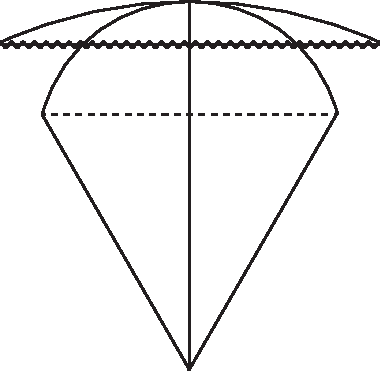
\includegraphics[width=0.57\textwidth]{images/LH035,02,01_273-d1.pdf}
%\\
%\noindent \centering [\textit{Fig. 1}]
\end{minipage}
\hspace*{17,3mm}
\begin{minipage}[c]{0.5\textwidth}
%\hspace*{-5mm}
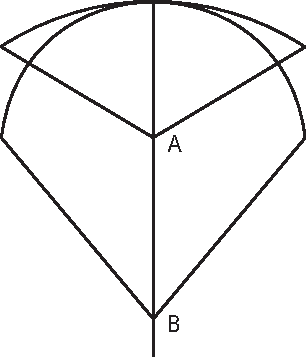
\includegraphics[width=0.57\textwidth]{images/LH035,02,01_273-d2.pdf}
%\\
%\noindent \centering [\textit{Fig. 2}]
\end{minipage}
\pend
\vspace{2mm}
\pstart
\noindent
%\vspace*{3mm}
\hspace*{23.5mm} [\textit{Fig. 1}]\hspace*{62.5mm} [\textit{Fig. 2}]
\vspace*{0.8em}
\pend
\pstart
\noindent
\begin{center}
\hspace{13mm}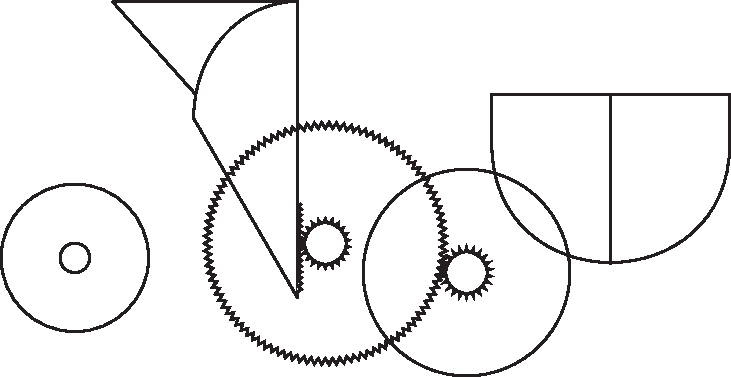
\includegraphics[width=0.6\textwidth]{images/LH035,02,01_273-d3.pdf}\newline
[\textit{Fig. 3}]
\end{center}
\pend
\newpage
\pstart
\noindent\lbrack273~v\textsuperscript{o}\rbrack
\pend
\pstart
\noindent
\centering
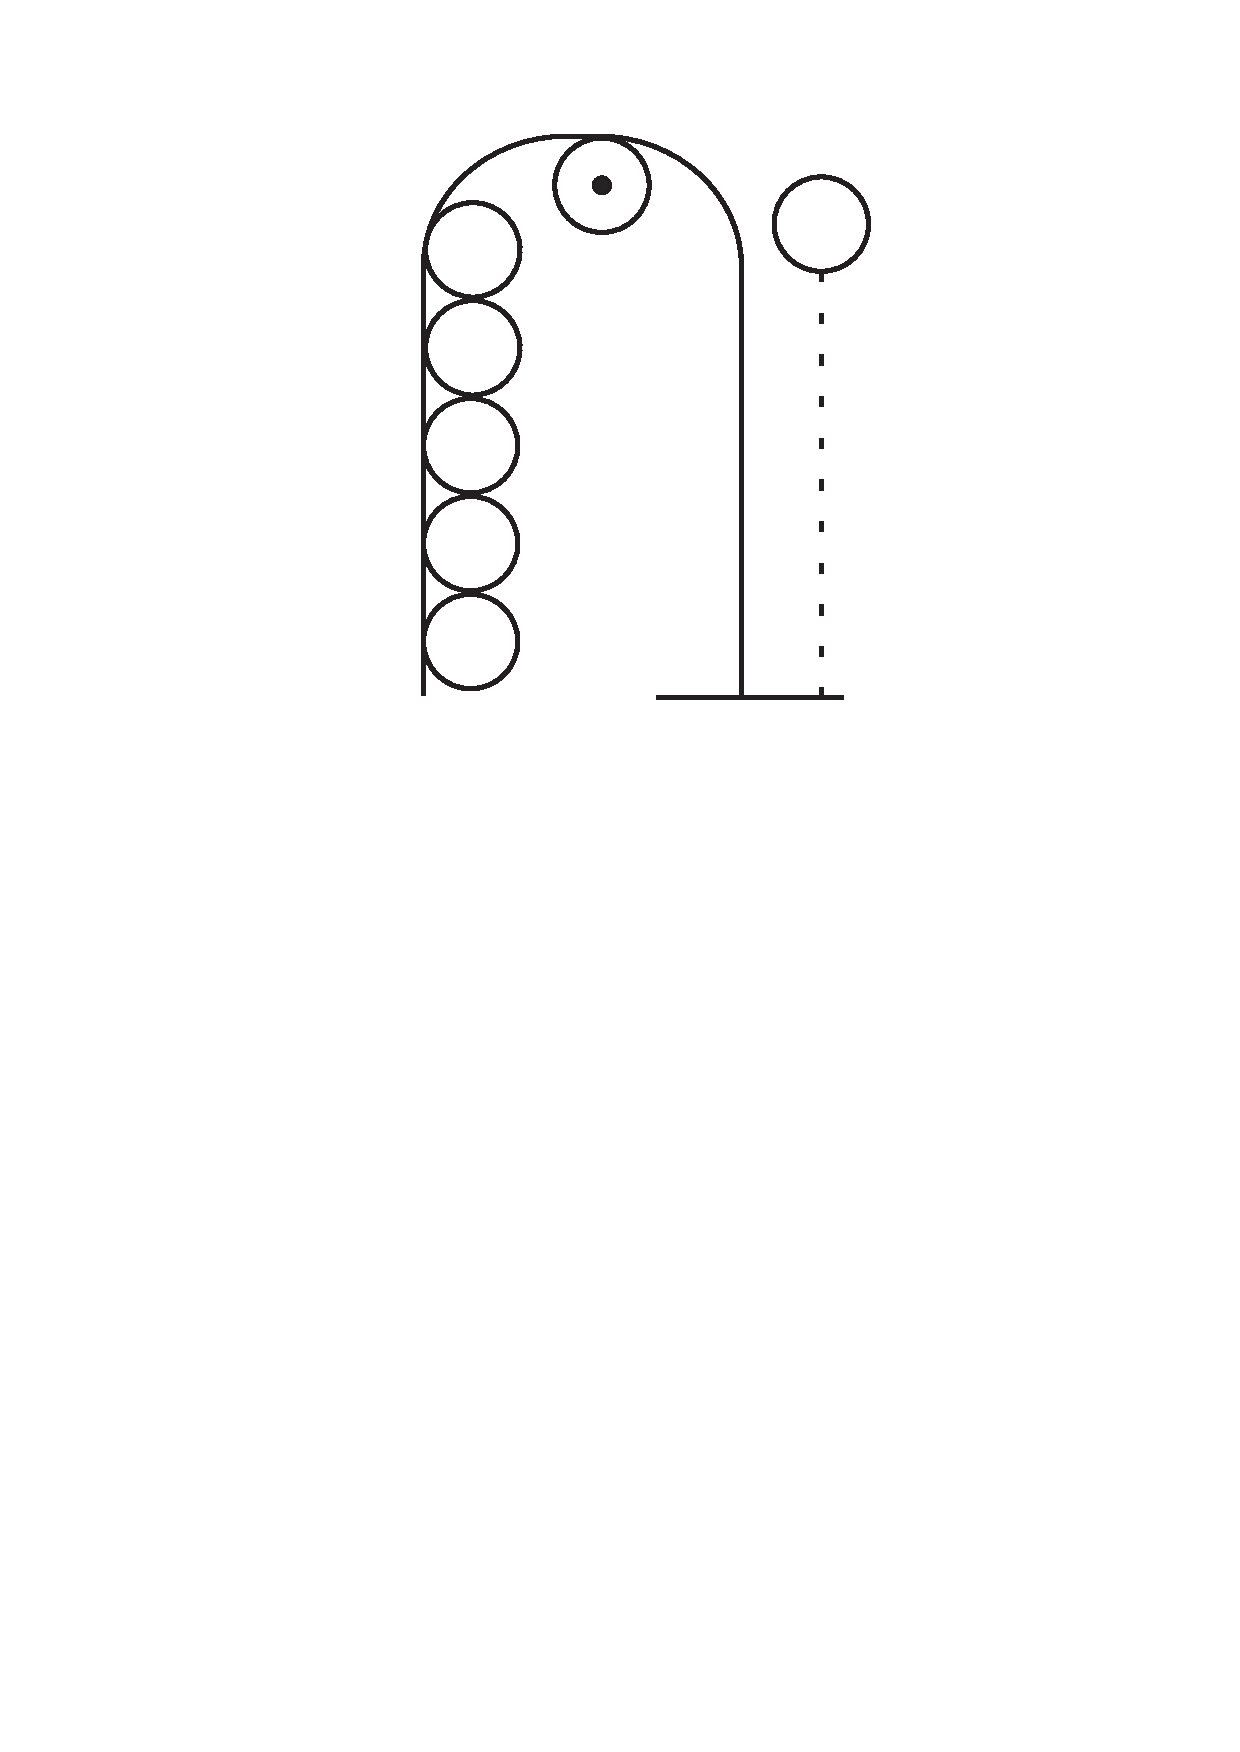
\includegraphics[trim = 0mm -2mm 0mm 0mm, clip, width=0.2\textwidth]{images/LH035,02,01_273-d4.pdf}\\
\centering[\textit{Fig. 4}]
\pend
\vspace{1.4em}
\pstart
\noindent
\centering
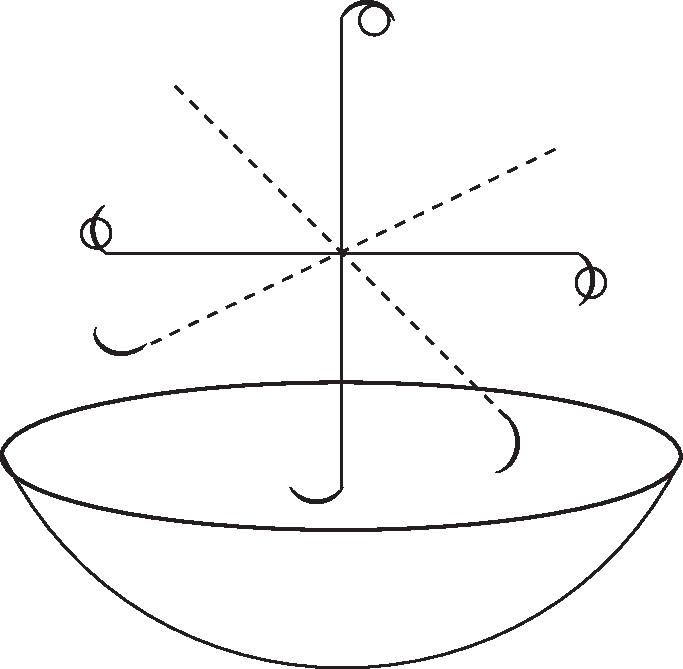
\includegraphics[trim = 0mm -2mm 0mm 0mm, clip, width=0.4\textwidth]{images/LH035,02,01_273-d5.pdf}\\
\centering
[\textit{Fig. 5}]\setline{6}
\pend
\vspace{1.4em}
\pstart
\noindent
\centering
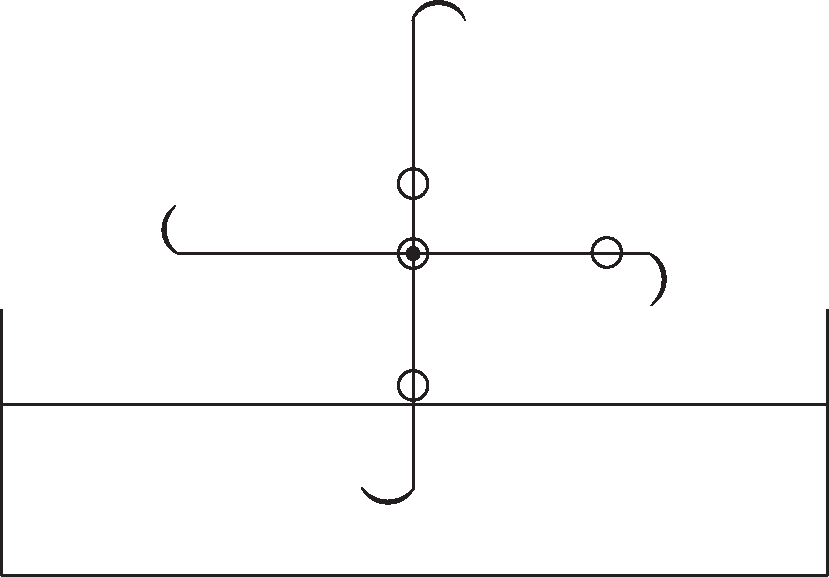
\includegraphics[trim = 0mm -2mm 0mm 0mm, clip, width=0.5\textwidth]{images/LH035,02,01_273-d6.pdf}\\
\centering
[\textit{Fig. 6}]
\pend
\newpage
\pstart
\noindent
\centering
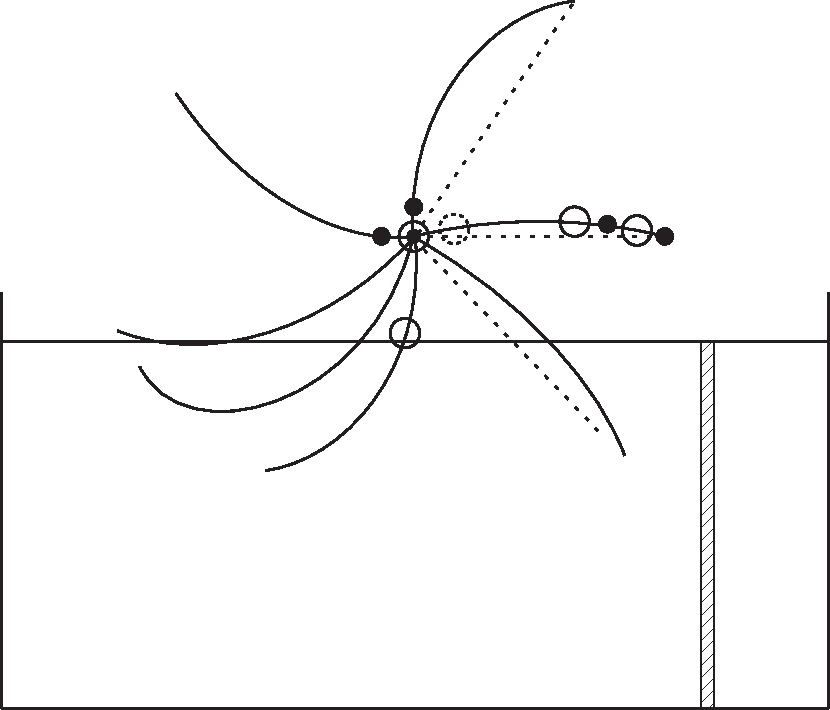
\includegraphics[trim = 0mm -2mm 0mm 0mm, clip, width=0.6\textwidth]{images/LH035,02,01_273-d7.pdf}\\
\centering
[\textit{Fig. 7}]
\pend
